\documentclass[../main.tex]{subfiles}

\begin{document}
\section*{Instalaciones y Configuraciones}
\section{VirtualBox}
\subsection{instalación}

\subsection{Guest Additions}
https://www.makeuseof.com/tag/virtualbox-guest-additions-what-they-are-and-how-to-install-them/

\subsection{configuración de la red de los equipos:}
se crea una conexión de tipo \textit{bridge }y se le da una IP fija a cada equipo, de esta manera las VM tienen conexión a Internet y una red dedicada.
\begin{list}{·}{}
	\item mint00 192.168.1.100
	\item mint01 192.168.1.101
	\item mint02 192.168.1.102
	\item mint03 192.168.1.103
\end{list}
\section{Instalación de Ansible and sshpass}
Installing Ansible and sshpass. checking ansible version
%formato de consola
\lstconsolestyle
\begin{lstlisting}
	tfg@mint01:~$ sudo apt update && sudo apt install software-properties-common && sudo add-apt-repository --yes ppa:ansible/ansible && sudo apt install ansible
	Hit:1 http://mirror.tedra.es/ubuntu jammy InRelease
	Hit:2 http://mirror.tedra.es/ubuntu jammy-updates InRelease                    
	Hit:3 http://mirror.tedra.es/ubuntu jammy-backports InRelease                  
	Get:4 http://security.ubuntu.com/ubuntu jammy-security InRelease [110 kB]      
	Ign:5 https://mirrors.ptisp.pt/linuxmint vera InRelease                        
	Hit:6 https://mirrors.ptisp.pt/linuxmint vera Release                          
	Hit:8 https://download.sublimetext.com apt/stable/ InRelease                   
	Get:9 http://security.ubuntu.com/ubuntu jammy-security/main amd64 DEP-11 Metadata [41,4 kB]
	Get:10 http://security.ubuntu.com/ubuntu jammy-security/universe amd64 DEP-11 Metadata [18,5 kB]
	Fetched 170 kB in 1s (214 kB/s)              
	Reading package lists... Done
	Building dependency tree... Done
	Reading state information... Done
	7 packages can be upgraded. Run 'apt list --upgradable' to see them.
	W: https://download.sublimetext.com/apt/stable/InRelease: Key is stored in legacy trusted.gpg keyring (/etc/apt/trusted.gpg), see the DEPRECATION section in apt-key(8) for details.
	Reading package lists... Done
	Building dependency tree... Done
	Reading state information... Done
	The following NEW packages will be installed:
	software-properties-common
	0 upgraded, 1 newly installed, 0 to remove and 7 not upgraded.
	Need to get 9.712 B of archives.
	After this operation, 16,4 kB of additional disk space will be used.
	Get:1 https://mirrors.ptisp.pt/linuxmint vera/upstream amd64 software-properties-common all 2.2.1 [9.712 B]
	Fetched 9.712 B in 0s (26,5 kB/s)                      
	Selecting previously unselected package software-properties-common.
	(Reading database ... 610456 files and directories currently installed.)
	Preparing to unpack .../software-properties-common_2.2.1_all.deb ...
	Unpacking software-properties-common (2.2.1) ...
	Setting up software-properties-common (2.2.1) ...
	You are about to add the following PPA:
	Ansible is a radically simple IT automation platform that makes your applications and systems easier to deploy. Avoid writing scripts or custom code to deploy and update your applications automate in a language that approaches plain English, using SSH, with no agents to install on remote systems.
	
	http://ansible.com/
	
	If you face any issues while installing Ansible PPA, file an issue here:
	https://github.com/ansible-community/ppa/issues
	More info: https://launchpad.net/~ansible/+archive/ubuntu/ansible
	gpg: directory '/root/.gnupg' created
	gpg: keybox '/root/.gnupg/pubring.kbx' created
	gpg: /root/.gnupg/trustdb.gpg: trustdb created
	gpg: keybox '/etc/apt/keyrings/6125E2A8C77F2818FB7BD15B93C4A3FD7BB9C367.keyring' created
	gpg: key 93C4A3FD7BB9C367: public key "Launchpad PPA for Ansible, Inc." imported
	gpg: Total number processed: 1
	gpg:               imported: 1
	Reading package lists... Done
	Building dependency tree... Done
	Reading state information... Done
	The following additional packages will be installed:
	python-babel-localedata python3-argcomplete python3-babel python3-distutils
	python3-dnspython python3-jinja2 python3-jmespath python3-kerberos
	python3-lib2to3 python3-libcloud python3-lockfile python3-ntlm-auth
	python3-pycryptodome python3-requests-kerberos python3-requests-ntlm
	python3-requests-toolbelt python3-selinux python3-simplejson python3-tz
	python3-winrm python3-xmltodict
	Suggested packages:
	cowsay sshpass python3-sniffio python3-trio python-jinja2-doc
	python-lockfile-doc
	The following NEW packages will be installed:
	ansible python-babel-localedata python3-argcomplete python3-babel
	python3-distutils python3-dnspython python3-jinja2 python3-jmespath
	python3-kerberos python3-lib2to3 python3-libcloud python3-lockfile
	python3-ntlm-auth python3-pycryptodome python3-requests-kerberos
	python3-requests-ntlm python3-requests-toolbelt python3-selinux
	python3-simplejson python3-tz python3-winrm python3-xmltodict
	0 upgraded, 22 newly installed, 0 to remove and 7 not upgraded.
	Need to get 26,1 MB of archives.
	After this operation, 259 MB of additional disk space will be used.
	Do you want to continue? [Y/n] Y
	Get:1 http://mirror.tedra.es/ubuntu jammy/main amd64 python-babel-localedata all 2.8.0+dfsg.1-7 [4.982 kB]
	Get:2 http://mirror.tedra.es/ubuntu jammy-updates/main amd64 python3-tz all 2022.1-1ubuntu0.22.04.0 [33,4 kB]
	Get:3 http://mirror.tedra.es/ubuntu jammy/main amd64 python3-babel all 2.8.0+dfsg.1-7 [85,1 kB]
	Get:4 http://mirror.tedra.es/ubuntu jammy/main amd64 python3-jinja2 all 3.0.3-1 [108 kB]
	Get:5 http://mirror.tedra.es/ubuntu jammy/main amd64 python3-pycryptodome amd64 3.11.0+dfsg1-3build1 [1.027 kB]
	Get:6 http://mirror.tedra.es/ubuntu jammy-updates/main amd64 python3-lib2to3 all 3.10.6-1~22.04 [77,6 kB]
	Get:7 http://mirror.tedra.es/ubuntu jammy-updates/main amd64 python3-distutils all 3.10.6-1~22.04 [139 kB]
	Get:8 http://mirror.tedra.es/ubuntu jammy/main amd64 python3-dnspython all 2.1.0-1ubuntu1 [123 kB]
	Get:9 http://mirror.tedra.es/ubuntu jammy/universe amd64 ansible all 2.10.7+merged+base+2.10.8+dfsg-1 [17,5 MB]
	Get:10 http://mirror.tedra.es/ubuntu jammy/universe amd64 python3-argcomplete all 1.8.1-1.5 [27,2 kB]
	Get:11 http://mirror.tedra.es/ubuntu jammy/main amd64 python3-jmespath all 0.10.0-1 [21,7 kB]
	Get:12 http://mirror.tedra.es/ubuntu jammy/universe amd64 python3-kerberos amd64 1.1.14-3.1build5 [23,0 kB]
	Get:13 http://mirror.tedra.es/ubuntu jammy/main amd64 python3-lockfile all 1:0.12.2-2.2 [14,6 kB]
	Get:14 http://mirror.tedra.es/ubuntu jammy/main amd64 python3-simplejson amd64 3.17.6-1build1 [54,7 kB]
	Get:15 http://mirror.tedra.es/ubuntu jammy/universe amd64 python3-libcloud all 3.2.0-2 [1.554 kB]
	Get:16 http://mirror.tedra.es/ubuntu jammy/universe amd64 python3-ntlm-auth all 1.4.0-1 [20,4 kB]
	Get:17 http://mirror.tedra.es/ubuntu jammy/universe amd64 python3-requests-kerberos all 0.12.0-2 [11,9 kB]
	Get:18 http://mirror.tedra.es/ubuntu jammy/universe amd64 python3-requests-ntlm all 1.1.0-1.1 [6.160 B]
	Get:19 http://mirror.tedra.es/ubuntu jammy/main amd64 python3-requests-toolbelt all 0.9.1-1 [38,0 kB]
	Get:20 http://mirror.tedra.es/ubuntu jammy/universe amd64 python3-selinux amd64 3.3-1build2 [159 kB]
	Get:21 http://mirror.tedra.es/ubuntu jammy/universe amd64 python3-xmltodict all 0.12.0-2 [12,6 kB]
	Get:22 http://mirror.tedra.es/ubuntu jammy/universe amd64 python3-winrm all 0.3.0-2 [21,7 kB]
	Fetched 26,1 MB in 3s (8.628 kB/s)   
	Selecting previously unselected package python-babel-localedata.
	(Reading database ... 610459 files and directories currently installed.)
	Preparing to unpack .../00-python-babel-localedata_2.8.0+dfsg.1-7_all.deb ...
	Unpacking python-babel-localedata (2.8.0+dfsg.1-7) ...
	Selecting previously unselected package python3-tz.
	Preparing to unpack .../01-python3-tz_2022.1-1ubuntu0.22.04.0_all.deb ...
	Unpacking python3-tz (2022.1-1ubuntu0.22.04.0) ...
	Selecting previously unselected package python3-babel.
	Preparing to unpack .../02-python3-babel_2.8.0+dfsg.1-7_all.deb ...
	Unpacking python3-babel (2.8.0+dfsg.1-7) ...
	Selecting previously unselected package python3-jinja2.
	Preparing to unpack .../03-python3-jinja2_3.0.3-1_all.deb ...
	Unpacking python3-jinja2 (3.0.3-1) ...
	Selecting previously unselected package python3-pycryptodome.
	Preparing to unpack .../04-python3-pycryptodome_3.11.0+dfsg1-3build1_amd64.deb .
	..
	Unpacking python3-pycryptodome (3.11.0+dfsg1-3build1) ...
	Selecting previously unselected package python3-lib2to3.
	Preparing to unpack .../05-python3-lib2to3_3.10.6-1~22.04_all.deb ...
	Unpacking python3-lib2to3 (3.10.6-1~22.04) ...
	Selecting previously unselected package python3-distutils.
	Preparing to unpack .../06-python3-distutils_3.10.6-1~22.04_all.deb ...
	Unpacking python3-distutils (3.10.6-1~22.04) ...
	Selecting previously unselected package python3-dnspython.
	Preparing to unpack .../07-python3-dnspython_2.1.0-1ubuntu1_all.deb ...
	Unpacking python3-dnspython (2.1.0-1ubuntu1) ...
	Selecting previously unselected package ansible.
	Preparing to unpack .../08-ansible_2.10.7+merged+base+2.10.8+dfsg-1_all.deb ...
	Unpacking ansible (2.10.7+merged+base+2.10.8+dfsg-1) ...
	Selecting previously unselected package python3-argcomplete.
	Preparing to unpack .../09-python3-argcomplete_1.8.1-1.5_all.deb ...
	Unpacking python3-argcomplete (1.8.1-1.5) ...
	Selecting previously unselected package python3-jmespath.
	Preparing to unpack .../10-python3-jmespath_0.10.0-1_all.deb ...
	Unpacking python3-jmespath (0.10.0-1) ...
	Selecting previously unselected package python3-kerberos.
	Preparing to unpack .../11-python3-kerberos_1.1.14-3.1build5_amd64.deb ...
	Unpacking python3-kerberos (1.1.14-3.1build5) ...
	Selecting previously unselected package python3-lockfile.
	Preparing to unpack .../12-python3-lockfile_1%3a0.12.2-2.2_all.deb ...
	Unpacking python3-lockfile (1:0.12.2-2.2) ...
	Selecting previously unselected package python3-simplejson.
	Preparing to unpack .../13-python3-simplejson_3.17.6-1build1_amd64.deb ...
	Unpacking python3-simplejson (3.17.6-1build1) ...
	Selecting previously unselected package python3-libcloud.
	Preparing to unpack .../14-python3-libcloud_3.2.0-2_all.deb ...
	Unpacking python3-libcloud (3.2.0-2) ...
	Selecting previously unselected package python3-ntlm-auth.
	Preparing to unpack .../15-python3-ntlm-auth_1.4.0-1_all.deb ...
	Unpacking python3-ntlm-auth (1.4.0-1) ...
	Selecting previously unselected package python3-requests-kerberos.
	Preparing to unpack .../16-python3-requests-kerberos_0.12.0-2_all.deb ...
	Unpacking python3-requests-kerberos (0.12.0-2) ...
	Selecting previously unselected package python3-requests-ntlm.
	Preparing to unpack .../17-python3-requests-ntlm_1.1.0-1.1_all.deb ...
	Unpacking python3-requests-ntlm (1.1.0-1.1) ...
	Selecting previously unselected package python3-requests-toolbelt.
	Preparing to unpack .../18-python3-requests-toolbelt_0.9.1-1_all.deb ...
	Unpacking python3-requests-toolbelt (0.9.1-1) ...
	Selecting previously unselected package python3-selinux.
	Preparing to unpack .../19-python3-selinux_3.3-1build2_amd64.deb ...
	Unpacking python3-selinux (3.3-1build2) ...
	Selecting previously unselected package python3-xmltodict.
	Preparing to unpack .../20-python3-xmltodict_0.12.0-2_all.deb ...
	Unpacking python3-xmltodict (0.12.0-2) ...
	Selecting previously unselected package python3-winrm.
	Preparing to unpack .../21-python3-winrm_0.3.0-2_all.deb ...
	Unpacking python3-winrm (0.3.0-2) ...
	Setting up python3-lockfile (1:0.12.2-2.2) ...
	Setting up python3-requests-toolbelt (0.9.1-1) ...
	Setting up python3-ntlm-auth (1.4.0-1) ...
	Setting up python3-pycryptodome (3.11.0+dfsg1-3build1) ...
	Setting up python3-kerberos (1.1.14-3.1build5) ...
	Setting up python3-tz (2022.1-1ubuntu0.22.04.0) ...
	Setting up python-babel-localedata (2.8.0+dfsg.1-7) ...
	Setting up python3-simplejson (3.17.6-1build1) ...
	Setting up python3-xmltodict (0.12.0-2) ...
	Setting up python3-jmespath (0.10.0-1) ...
	Setting up python3-requests-kerberos (0.12.0-2) ...
	Setting up python3-dnspython (2.1.0-1ubuntu1) ...
	Setting up python3-selinux (3.3-1build2) ...
	Setting up python3-argcomplete (1.8.1-1.5) ...
	Setting up python3-lib2to3 (3.10.6-1~22.04) ...
	Setting up python3-distutils (3.10.6-1~22.04) ...
	Setting up python3-requests-ntlm (1.1.0-1.1) ...
	Setting up python3-babel (2.8.0+dfsg.1-7) ...
	update-alternatives: using /usr/bin/pybabel-python3 to provide /usr/bin/pybabel 
	(pybabel) in auto mode
	Setting up python3-libcloud (3.2.0-2) ...
	Setting up python3-jinja2 (3.0.3-1) ...
	Setting up python3-winrm (0.3.0-2) ...
	Setting up ansible (2.10.7+merged+base+2.10.8+dfsg-1) ...
	Processing triggers for man-db (2.10.2-1) ...
	tfg@mint00:~$ ansible --version
	ansible 2.10.8
	config file = None
	configured module search path = ['/home/tfg/.ansible/plugins/modules', '/usr/share/ansible/plugins/modules']
	ansible python module location = /usr/lib/python3/dist-packages/ansible
	executable location = /usr/bin/ansible
	python version = 3.10.6 (main, Mar 10 2023, 10:55:28) [GCC 11.3.0]
	
	tfg@Mint03:~$ sudo apt-get install sshpass
	[sudo] password for tfg:        
	Reading package lists... Done
	Building dependency tree... Done
	Reading state information... Done
	The following NEW packages will be installed:
	sshpass
	0 upgraded, 1 newly installed, 0 to remove and 8 not upgraded.
	Need to get 11,7 kB of archives.
	After this operation, 35,8 kB of additional disk space will be used.
	Get:1 http://mirror.tedra.es/ubuntu jammy/universe amd64 sshpass amd64 1.09-1 [11,7 kB]
	Fetched 11,7 kB in 0s (214 kB/s)    
	Selecting previously unselected package sshpass.
	(Reading database ... 649950 files and directories currently installed.)
	Preparing to unpack .../sshpass_1.09-1_amd64.deb ...
	Unpacking sshpass (1.09-1) ...
	Setting up sshpass (1.09-1) ...
	Processing triggers for man-db (2.10.2-1) ...
\end{lstlisting}
instalar dependencias de ansible
\begin{lstlisting}
sudo apt-get install ansible-core
\end{lstlisting}


\section{Instalación de de kubeadm}
Para poder utilizar docker necesitamos instalar varios paquetes. Estos son Docker Engine, kubectl, kubelet y kubeadm. Pasamos a instalar cada uno individualmente. 

\subsection{instalación kubectl}
Hay que descargarse la última release:

\begin{lstlisting}
 curl -LO https://storage.googleapis.com/kubernetes-release/release/$(curl -s https://storage.googleapis.com/kubernetes-release/release/stable.txt)/bin/linux/amd64/kubectl
\end{lstlisting}

Para que el archivo sea ejecutable utilizamos chmod.
\begin{lstlisting}
chmod +x kubectl
\end{lstlisting}
se mueve el archivo binario al path del usuario para ejecutarlo directamente desde la consola.

\begin{lstlisting}
sudo mv kubectl /usr/local/bin/kubectl
\end{lstlisting}
 
Se comprueba que la instalación ha sido correcta mediante el comando kubectl. Debe devolver la ayuda del mismo.

\begin{lstlisting}     
 tfg@mint01:~$ kubectl 
 kubectl controls the Kubernetes cluster manager.
 
 Find more information at: https://kubernetes.io/docs/reference/kubectl/
 
 Basic Commands (Beginner):
 create          Create a resource from a file or from stdin
 expose          Take a replication controller, service, deployment or pod and
 expose it as a new Kubernetes service
 run             Run a particular image on the cluster
 set             Set specific features on objects
 
 Basic Commands (Intermediate):
 explain         Get documentation for a resource
 get             Display one or many resources
 edit            Edit a resource on the server
 delete          Delete resources by file names, stdin, resources and names, or
 by resources and label selector
 
 Deploy Commands:
 rollout         Manage the rollout of a resource
 scale           Set a new size for a deployment, replica set, or replication
 controller
 autoscale       Auto-scale a deployment, replica set, stateful set, or
 replication controller
 
 Cluster Management Commands:
 certificate     Modify certificate resources.
 cluster-info    Display cluster information
 top             Display resource (CPU/memory) usage
 cordon          Mark node as unschedulable
 uncordon        Mark node as schedulable
 drain           Drain node in preparation for maintenance
 taint           Update the taints on one or more nodes
 
 Troubleshooting and Debugging Commands:
 describe        Show details of a specific resource or group of resources
 logs            Print the logs for a container in a pod
 attach          Attach to a running container
 exec            Execute a command in a container
 port-forward    Forward one or more local ports to a pod
 proxy           Run a proxy to the Kubernetes API server
 cp              Copy files and directories to and from containers
 auth            Inspect authorization
 debug           Create debugging sessions for troubleshooting workloads and
 nodes
 events          List events
 
 Advanced Commands:
 diff            Diff the live version against a would-be applied version
 apply           Apply a configuration to a resource by file name or stdin
 patch           Update fields of a resource
 replace         Replace a resource by file name or stdin
 wait            Experimental: Wait for a specific condition on one or many
 resources
 kustomize       Build a kustomization target from a directory or URL
 
 Settings Commands:
 label           Update the labels on a resource
 annotate        Update the annotations on a resource
 completion      Output shell completion code for the specified shell (bash,
 zsh, fish, or powershell)
 
 Other Commands:
 api-resources   Print the supported API resources on the server
 api-versions    Print the supported API versions on the server, in the form of
 "group/version"
 config          Modify kubeconfig files
 plugin          Provides utilities for interacting with plugins
 version         Print the client and server version information
 
 Usage:
 kubectl [flags] [options]
 
 Use "kubectl <command> --help" for more information about a given command.
 Use "kubectl options" for a list of global command-line options (applies to all
 commands).
 \end{lstlisting}
 
Se pueden ejecutar los 4 comando a la vez mediante la instrucción:
\begin{lstlisting} 
  curl -LO https://storage.googleapis.com/kubernetes-release/release/$(curl -s https://storage.googleapis.com/kubernetes-release/release/stable.txt)/bin/linux/amd64/kubectl &&  chmod +x ./kubectl && sudo mv ./kubectl /usr/local/bin/kubectl && kubectl
\end{lstlisting}
\subsection{Instalación de docker Engine}
\subsubsection{Configuración del repositorio}
Primero, se actualiza el paquete apt y se instalan los certificados necesarios
\begin{lstlisting} 
sudo apt-get update
sudo apt-get install \
ca-certificates \
curl \
gnupg
\end{lstlisting} 

Se debe añadir la GPG key oficial de docker a los keyrings.
\begin{lstlisting}
sudo install -m 0755 -d /etc/apt/keyrings
curl -fsSL https://download.docker.com/linux/ubuntu/gpg | sudo gpg --dearmor -o /etc/apt/keyrings/docker.gpg
sudo chmod a+r /etc/apt/keyrings/docker.gpg
\end{lstlisting}

Se añade el repositorio para la descarga y configuración de docker al archivo de configuración de repositorios para docker.
\begin{lstlisting}
echo \
"deb [arch="$(dpkg --print-architecture)" signed-by=/etc/apt/keyrings/docker.gpg] https://download.docker.com/linux/ubuntu \
"$(. /etc/os-release && echo "$VERSION_CODENAME")" stable" | \
sudo tee /etc/apt/sources.list.d/docker.list > /dev/null 
\end{lstlisting}

Una vez configurado el repositorio, se ejecuta del comando apt-get update.
\begin{lstlisting}
sudo apt-get update
\end{lstlisting}
En este punto puede ser que haya un error al no existir una versión de Docker para la distribución de linux sobre la que estamos trabajando.

\begin{lstlisting}
sudo apt-get update 
Ign:1 https://ftp.crifo.org/mint-packages vera InRelease
Hit:2 https://ppa.launchpadcontent.net/ansible/ansible/ubuntu jammy InRelease  
Hit:3 https://ftp.crifo.org/mint-packages vera Release                         
Hit:4 http://archive.ubuntu.com/ubuntu jammy InRelease                         
Hit:5 http://security.ubuntu.com/ubuntu jammy-security InRelease               
Ign:7 https://download.docker.com/linux/ubuntu vera InRelease                  
Hit:8 http://archive.ubuntu.com/ubuntu jammy-updates InRelease                 
Hit:9 http://archive.ubuntu.com/ubuntu jammy-backports InRelease               
Err:10 https://download.docker.com/linux/ubuntu vera Release                   
404  Not Found [IP: 18.67.240.122 443]
Hit:11 https://download.sublimetext.com apt/stable/ InRelease
Reading package lists... Done
E: The repository 'https://download.docker.com/linux/ubuntu vera Release' does not have a Release file.
N: Updating from such a repository can't be done securely, and is therefore disabled by default.
N: See apt-secure(8) manpage for repository creation and user configuration details.
\end{lstlisting}

De darse el caso, se debe editar el archivo \textit{/etc/apt/sources.list.d/docker.list} con la versión de docker disponible más cercana a la que está en ejecución. Para ello hay que buscar en \textit{https://download.docker.com/linux/ubuntu/dists/} las distribuciones para las que docker tiene releases y se elige la que más convenga. Para saber qué distribución es la del SO en uso, se revisa el archivo \textit{/etc/os-release} y se elige el \textit{VERSION\_CODENAME} o el 
 \textit{UBUNTU\_CODENAME}.
 
Finalmente se instalan los paquetes necesarios para que docker funcione correctamente:
\begin{lstlisting}
sudo apt-get install docker-ce docker-ce-cli containerd.io docker-buildx-plugin docker-compose-plugin 
\end{lstlisting}
Se puede verificar la correcta instalción ejecutando un \textit{hello world} docker style.
\begin{lstlisting} 
sudo docker run hello-world
Unable to find image 'hello-world:latest' locally
latest: Pulling from library/hello-world
2db29710123e: Pull complete 
Digest: sha256:4e83453afed1b4fa1a3500525091dbfca6ce1e66903fd4c01ff015dbcb1ba33e
Status: Downloaded newer image for hello-world:latest

Hello from Docker!
This message shows that your installation appears to be working correctly.

To generate this message, Docker took the following steps:
1. The Docker client contacted the Docker daemon.
2. The Docker daemon pulled the "hello-world" image from the Docker Hub.
(amd64)
3. The Docker daemon created a new container from that image which runs the
executable that produces the output you are currently reading.
4. The Docker daemon streamed that output to the Docker client, which sent it
to your terminal.

To try something more ambitious, you can run an Ubuntu container with:
$ docker run -it ubuntu bash

Share images, automate workflows, and more with a free Docker ID:
https://hub.docker.com/

For more examples and ideas, visit:
https://docs.docker.com/get-started/
\end{lstlisting}

\subsubsection{Instalación de kubelet y kubeadm} 
El último paso antes de empezar a crear el clúster es instalar kubelet y kubeadm, para ello se ejecutan los siguientes comandos en la terminal \textbf{con un usuario con permisos de root}. 
\begin{lstlisting} 
apt-get update && apt-get install -y apt-transport-https

curl -s https://packages.cloud.google.com/apt/doc/apt-key.gpg | apt-key add -

cat <<EOF >/etc/apt/sources.list.d/kubernetes.list
deb http://apt.kubernetes.io/ kubernetes-xenial main
EOF

apt-get update

apt-get install -y kubelet kubeadm
\end{lstlisting}


\section{Creación del cluster}
El master va a ser el mint00. Accedemos a MV y ejecutamos la siguiente instrucción donde la IP configurada como \textit{apiserver-advertise-address} es la del adaptador que hace de bridge (Ver dirección MAC) en \ref{adaptador1} y \ref{adaptadorconfig} y la que queda como \textit{--pod-network-cidr} es la NAT. \ref{adaptador2}

\begin{figure}[!h]
	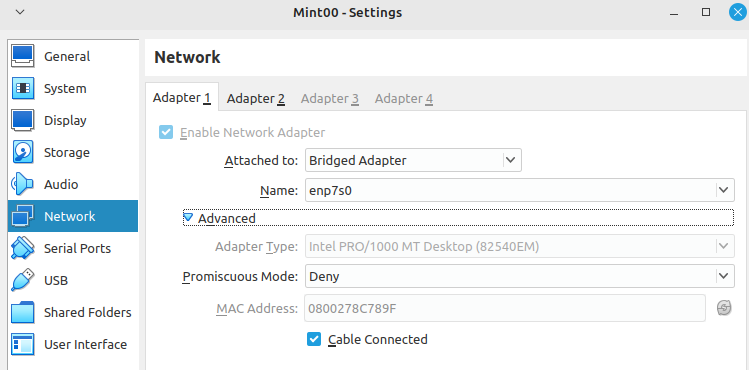
\includegraphics[scale=0.5]{00.png}
	\caption{Configuración Adaptador 1.}
	\label{adaptador1}
\end{figure} 
\begin{figure}[!h]
	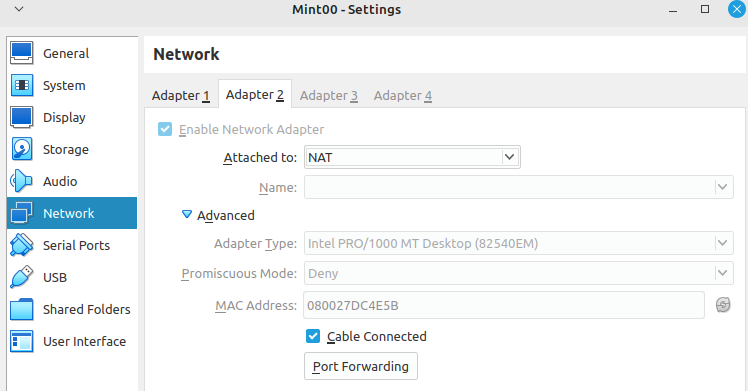
\includegraphics[scale=0.5]{01.png}
	\caption{Configuración Adaptador 2.}
	\label{adaptador2}
\end{figure} 
\begin{figure}[!h]
	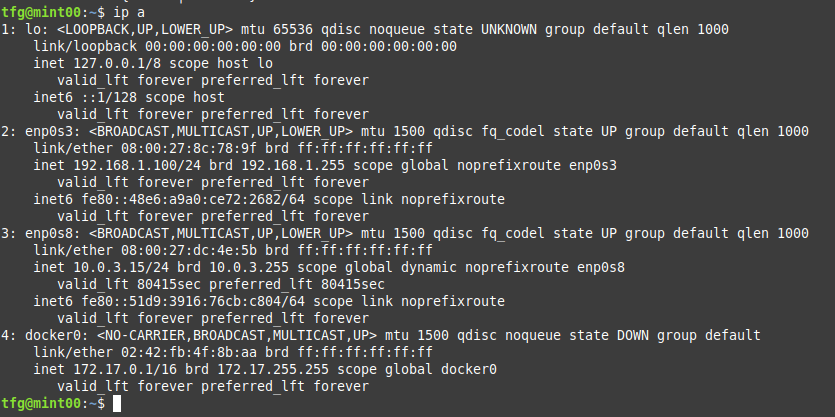
\includegraphics[scale=0.5]{02.png}
	\caption{Direcciones de los adaptadores en la Máquina Virtual.}
	\label{adaptadorconfig}
\end{figure} 


\begin{lstlisting} 
	sudo kubeadm init --apiserver-advertise-address 192.168.1.100 --pod-network-cidr=10.0.3.15
\end{lstlisting}
En este momento puede surgir un error. 
\begin{lstlisting}
	sudo kubeadm init --apiserver-advertise-address 192.168.1.100 --pod-network-cidr=10.0.3.15
	[sudo] password for tfg:
	[init] Using Kubernetes version: v1.27.1
	[preflight] Running pre-flight checks
	[WARNING Swap]: swap is enabled; production deployments should disable swap unless testing the NodeSwap feature gate of the kubelet
	error execution phase preflight: [preflight] Some fatal errors occurred:
	[ERROR CRI]: container runtime is not running: output: time="2023-05-06T17:35:28+02:00" level=fatal msg="validate service connection: CRI v1 runtime API is not implemented for endpoint \"unix:///var/run/containerd/containerd.sock\": rpc error: code = Unimplemented desc = unknown service runtime.v1.RuntimeService"
	, error: exit status 1
	[preflight] If you know what you are doing, you can make a check non-fatal with `--ignore-preflight-errors=...`
	To see the stack trace of this error execute with --v=5 or higher	
\end{lstlisting}
Esto es un error del paquete containerd que se puede resolver de la siguiente manera:
como usuario root, se elimina el paquete containerd, se actualiza e instala de nuevo el paquete, se elimina la configuración por defecto y se reinicia el programa.

\begin{lstlisting}
	apt remove containerd 
	apt update && apt install containerd.io 
	rm /etc/containerd/config.toml 
	systemctl restart containerd 
\end{lstlisting}

Una vez resuelto este inconveniente podemos iniciar el master. Para ello, usamos el comando y esperamos a que arranque satisfactoriamente. A continuación vemos algunas de las líneas de salida de la ejecución.

\begin{lstlisting}
	 sudo kubeadm init --apiserver-advertise-address 192.168.1.100 --pod-network-cidr=10.0.3.15
	 [init] Using Kubernetes version: v1.27.1
	 [preflight] Running pre-flight checks
	 [preflight] Pulling images required for setting up a Kubernetes cluster
	 [preflight] This might take a minute or two, depending on the speed of your internet connection
	 
	 [certs] apiserver serving cert is signed for DNS names [kubernetes kubernetes.default kubernetes.default.svc kubernetes.default.svc.cluster.local mint00] and IPs [10.96.0.1 192.168.1.100]
	 [apiclient] All control plane components are healthy after 4.001839 seconds
	 	 
	 Your Kubernetes control-plane has initialized successfully!
	 
	 To start using your cluster, you need to run the following as a regular user:
	 
	 mkdir -p $HOME/.kube
	 sudo cp -i /etc/kubernetes/admin.conf $HOME/.kube/config
	 sudo chown $(id -u):$(id -g) $HOME/.kube/config
	 
	 Alternatively, if you are the root user, you can run:
	 
	 export KUBECONFIG=/etc/kubernetes/admin.conf
	 
	 You should now deploy a pod network to the cluster.
	 Run "kubectl apply -f [podnetwork].yaml" with one of the options listed at:
	 https://kubernetes.io/docs/concepts/cluster-administration/addons/
	 
	 Then you can join any number of worker nodes by running the following on each as root:
	 
	 kubeadm join 192.168.1.100:6443 --token k79hza.63kxu2jlx6f6qzdb \
	 --discovery-token-ca-cert-hash sha256:83c9ec0ea6a42546598b01fa1a54f52f2bcdb2109395f3605772740922d788a0
\end{lstlisting}
Además muestra el comando a ejecutar para unir otros nodos a la red.
Antes de añadir los demás pods se deben ejecutar los siguientes comando sólo en el nodo master para guardar la configuración:
\begin{lstlisting}
	mkdir -p $HOME/.kube && sudo cp -i /etc/kubernetes/admin.conf $HOME/.kube/config && sudo chown $(id -u):$(id -g) $HOME/.kube/config
\end{lstlisting}

Puede ser que al intentar agregar los demás nodos muestre el error del paquete CRI como en el nodo master. Se resuelve de la misma manera. Deshabilitamos la memoria swap para que no muestre el warning y ejecutamos el comando.
\begin{lstlisting}
	sudo swapoff -a	 
	sudo kubeadm join 192.168.1.100:6443 --token k79hza.63kxu2jlx6f6qzdb \
	--discovery-token-ca-cert-hash sha256:83c9ec0ea6a42546598b01fa1a54f52f2bcdb2109395f3605772740922d788a0
\end{lstlisting}
Para comprobar que se han creado correctamente, se ejecuta el comando:
\begin{lstlisting}
	kubectl get nodes
\end{lstlisting}
Hace falta un paso extra que se ha realizado en este punto de la configuración. Se va a trabajar con fannel para configurar la red. Para ello es necesario descargarse la configuración escribiendo:
\begin{lstlisting}
	wget https://raw.githubusercontent.com/coreos/flannel/master/Documentation/kube-flannel.yml	
\end{lstlisting}
Una vez descargado, se debe modificar el archivo \ref{flannel}, añadiendo a la sección \textit{flanneld}, la interfaz correspondiente, en este caso se añade la línea \textit{- --iface=enp0s3} \ref{adaptadorconfig} con el identificador del adaptador configurado como bridge.

\begin{figure}[!h]
	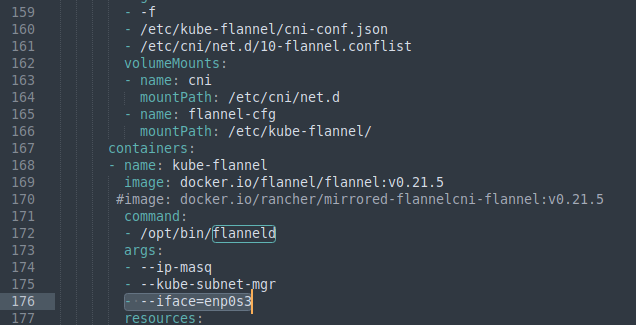
\includegraphics[scale=0.5]{03.png}
	\caption{kube-flannel.yml.}
	\label{flannel}
\end{figure} 
Una vez realizada toda la configuración correctamente, se observan los nodos agregados al cluster.

\begin{figure}[!h]
	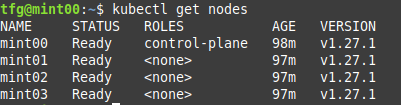
\includegraphics[scale=0.5]{04.png}
	\caption{Ejecución del comando get nodes.}
	\label{getNodes}
\end{figure} 
Se puede configurar 

\begin{lstlisting}
\end{lstlisting}

\begin{lstlisting}
\end{lstlisting}


\section{Instalar programas de obs}
\subsection{install obs studio}
\begin{lstlisting}
	
	args@BobPc02:\$ docker pull somatorio/obs-studio
	Using default tag: latest
	latest: Pulling from somatorio/obs-studio
	b3e1c725a85f: Pull complete 
	4daad8bdde31: Pull complete 
	63fe8c0068a8: Pull complete 
	4a70713c436f: Pull complete 
	bd842a2105a8: Pull complete 
	ad2d0b4ee955: Pull complete 
	Digest: sha256:583b32f6719ff422f70cc553d97968b34025f0bc3cc1e5495bcb46c7ea672fb3
	Status: Downloaded newer image for somatorio/obs-studio:latest
	docker.io/somatorio/obs-studio:latest
\end{lstlisting}

\begin{lstlisting}
	root@BobPc02:/home/args# sudo apt-get update && apt-get install -y obs-studio curl ffmpeg
\end{lstlisting}


\end{document}